\documentclass{ximera}
% nagekeken 20/08/2026
\title{Tribo-elektrisch effect}
\author{Daan Lipkens}

\begin{document}
\begin{abstract}
    Hoe objecten ladingen uitwisselen.
\end{abstract}
\maketitle
\section{Tribo-elektrisch effect}
\begin{remark}[foldable=true,title={Lading in een atoom}]\nl
Een atoom bestaat uit een kern van protonen en neutronen in het midden, omgeven door een elektronenwolk. Alleen de elektronen kunnen aan een atoom worden toegevoegd of ervan worden onttrokken; protonen worden nooit uitgewisseld.
\end{remark}

Omdat alle materie is opgebouwd uit atomen, en atomen op hun beurt uit elektronen, protonen en neutronen bestaan, bevat elke stof geladen deeltjes. In de meeste gevallen bevatten atomen evenveel protonen als elektronen. Wanneer een stof evenveel positieve als negatieve ladingen bevat, is ze elektrisch neutraal.

Een stof kan enkel een lading \textit{krijgen} wanneer er ladingen worden uitgewisseld. Een stof wordt negatief geladen wanneer ze extra elektronen opneemt, en positief geladen wanneer ze elektronen afstaat.

%-----------------
%Definitie tribo-elektisch effect
\begin{definition}[foldable=true,title={Tribo-elektrisch effect}]\nl
    Het \textbf{tribo-elektrisch effect} is een soort contactelektrificatie waarbij de materialen die met elkaar in contact komen tijdens het wrijven elektrische lading uitwisselen en zo elektrisch opgeladen worden.
\end{definition}
%------------------
\section{Tribo-elektrische reeks}
Wanneer je een materiaal dat hoger (meer links) in de tribo-elektrische reeks staat (zie figuur \ref{fig:tribo-elektrische-reeks}), wrijft tegen een materiaal dat lager (meer rechts) in de reeks staat, zal het hoger geplaatste materiaal elektronen afstaan en daardoor positief geladen worden. Het lager geplaatste materiaal neemt deze elektronen op en wordt negatief geladen.

%---------------------------------
% TRIBO-ELEKTRISCHE REEKS HORIZONTAAL
\begin{figure}[ht]
\centering
% \resizebox zorgt ervoor dat de pijl altijd netjes binnen de paginabreedte past
\resizebox{\textwidth}{!}{%
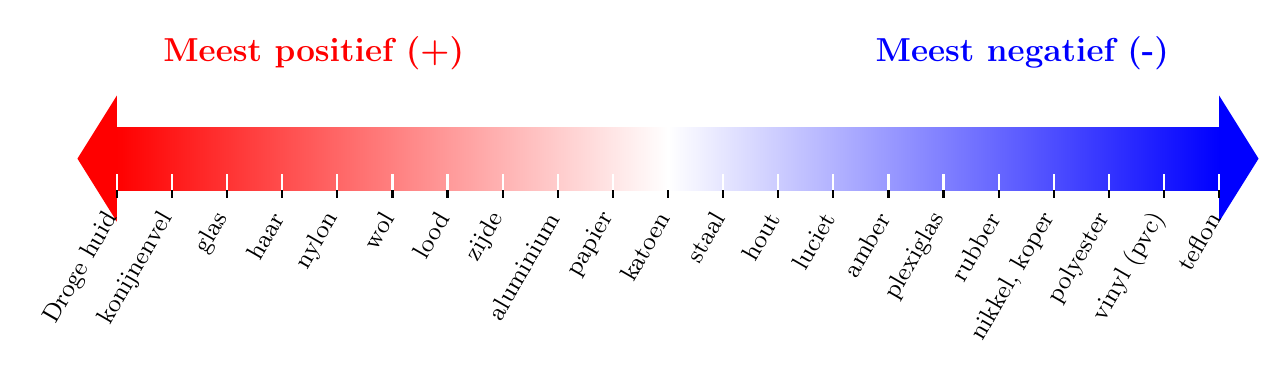
\begin{tikzpicture}
    % De gradient rechthoek (het midden van de pijl)
    \shade[left color=red, right color=blue, middle color=white] (0.5, -0.4) rectangle (14.5, 0.4);
    
    % Linker pijlpunt (rood, positief)
    \fill[red] (0.5, 0.8) -- (0, 0) -- (0.5, -0.8) -- cycle;
    
    % Rechter pijlpunt (blauw, negatief)
    \fill[blue] (14.5, 0.8) -- (15, 0) -- (14.5, -0.8) -- cycle;
    
    % Bijschriften boven de pijl
    \node[anchor=south, font=\bfseries\large, text=red] at (3, 1) {Meest positief (+)};
    \node[anchor=south, font=\bfseries\large, text=blue] at (12, 1) {Meest negatief (-)};
    
    % Materialen itereren
    % Let op: {nikkel, koper} staat tussen accolades zodat de komma de lijst niet breekt
    \foreach \materiaal [count=\i from 0] in {
        Droge huid, konijnenvel, glas, haar, nylon, wol, lood, zijde, aluminium, papier, 
        katoen, staal, hout, luciet, amber, plexiglas, rubber, {nikkel, koper}, polyester, vinyl (pvc), teflon
    } {
        % Witte streepjes in de pijl voor de afleesbaarheid
        \draw[thick, white] (0.5 + \i*0.7, -0.4) -- (0.5 + \i*0.7, -0.2);
        % Zwarte indicatorstreepjes onder de pijl
        \draw[thick, black] (0.5 + \i*0.7, -0.4) -- (0.5 + \i*0.7, -0.5);
        % Tekstlabels schuin (60 graden) onder de pijl
        \node[anchor=east, rotate=60, font=\small] at (0.5 + \i*0.7, -0.6) {\materiaal};
    }
\end{tikzpicture}%
}
\caption{Tribo-elektrische reeks}
\label{fig:tribo-elektrische-reeks}
\end{figure}
%------------------------
%-----------------------
% VB TRIBO ELEKTRISCHE REEKS
\begin{example}[expandable=true,title={Welke lading krijgen wol en zijde?}]\nl
Om te bepalen welke lading twee stoffen krijgen wanneer ze over elkaar wrijven, kunnen we de tribo-elektrische reeks raadplegen (zie figuur \ref{fig:tribo-elektrische-reeks}). Zo zal bij het wrijven van wol en zijde de wol positief geladen worden doordat deze elektronen afstaat, en de zijde negatief geladen worden omdat deze elektronen opneemt. We zien inderdaad dat wol hoger op de tribo-elektrische reeks staat dan zijde.
\begin{hint}
Dat beide materialen zich in het positieve deel van de reeks bevinden, maakt niet uit. Het is altijd de relatieve positie (de onderlinge verhouding) tussen de twee die bepaalt welke stof er positief en welke er negatief zal worden.
\end{hint}
\end{example}
%----------------------
%---------------
%QUIZ 3: TRIBO_ELEKTRISHCE REEKS
\begin{question}
    Je wrijft met rubber over een pvc-buis. Wat kun je zeggen over de lading van beide stoffen? Maak gebruik van figuur~\ref{fig:tribo-elektrische-reeks}. (a) Beide stoffen worden negatief geladen na het wrijven. (b) Rubber wordt positief geladen en pvc negatief geladen. (c) Rubber wordt negatief geladen en pvc positief geladen. (d) Beide stoffen worden positief geladen. (e) Met deze figuur kun je de soort lading niet bepalen. (f) Rubber en pvc kunnen niet tegen elkaar gewreven worden om lading uit te wisselen.
    \begin{onlineOnly}
        \begin{selectAll}
            \choice{$a$}
            \choice[correct]{$b$}
            \choice{$c$}
            \choice{$d$}
        \end{selectAll}
        \begin{solution}
        Rubber staat hoger (meer naar links) dan pvc in de tribo-elektrische reeks (zie figuur~\ref{fig:tribo-elektrische-reeks}). Rubber zal daardoor elektronen afstaan aan de pvc-buis en zo positief geladen worden. Het pvc neemt deze elektronen op en wordt hierdoor negatief geladen. 
        \end{solution}
    \end{onlineOnly}
\end{question}
%---------------

\end{document}